%%%%%%%%%%%%%%%%%%%%%%%%%%%%%%%%%%%%%%%%%%%%%%%%%%%%%%%%%%%%%%%%%%%%%%%%%%%%%%%%%%%%%%%%%%%%%%%%
\section{Model overview}
\label{sec: model}
 
\begin{figure}[htp]
 \centering
 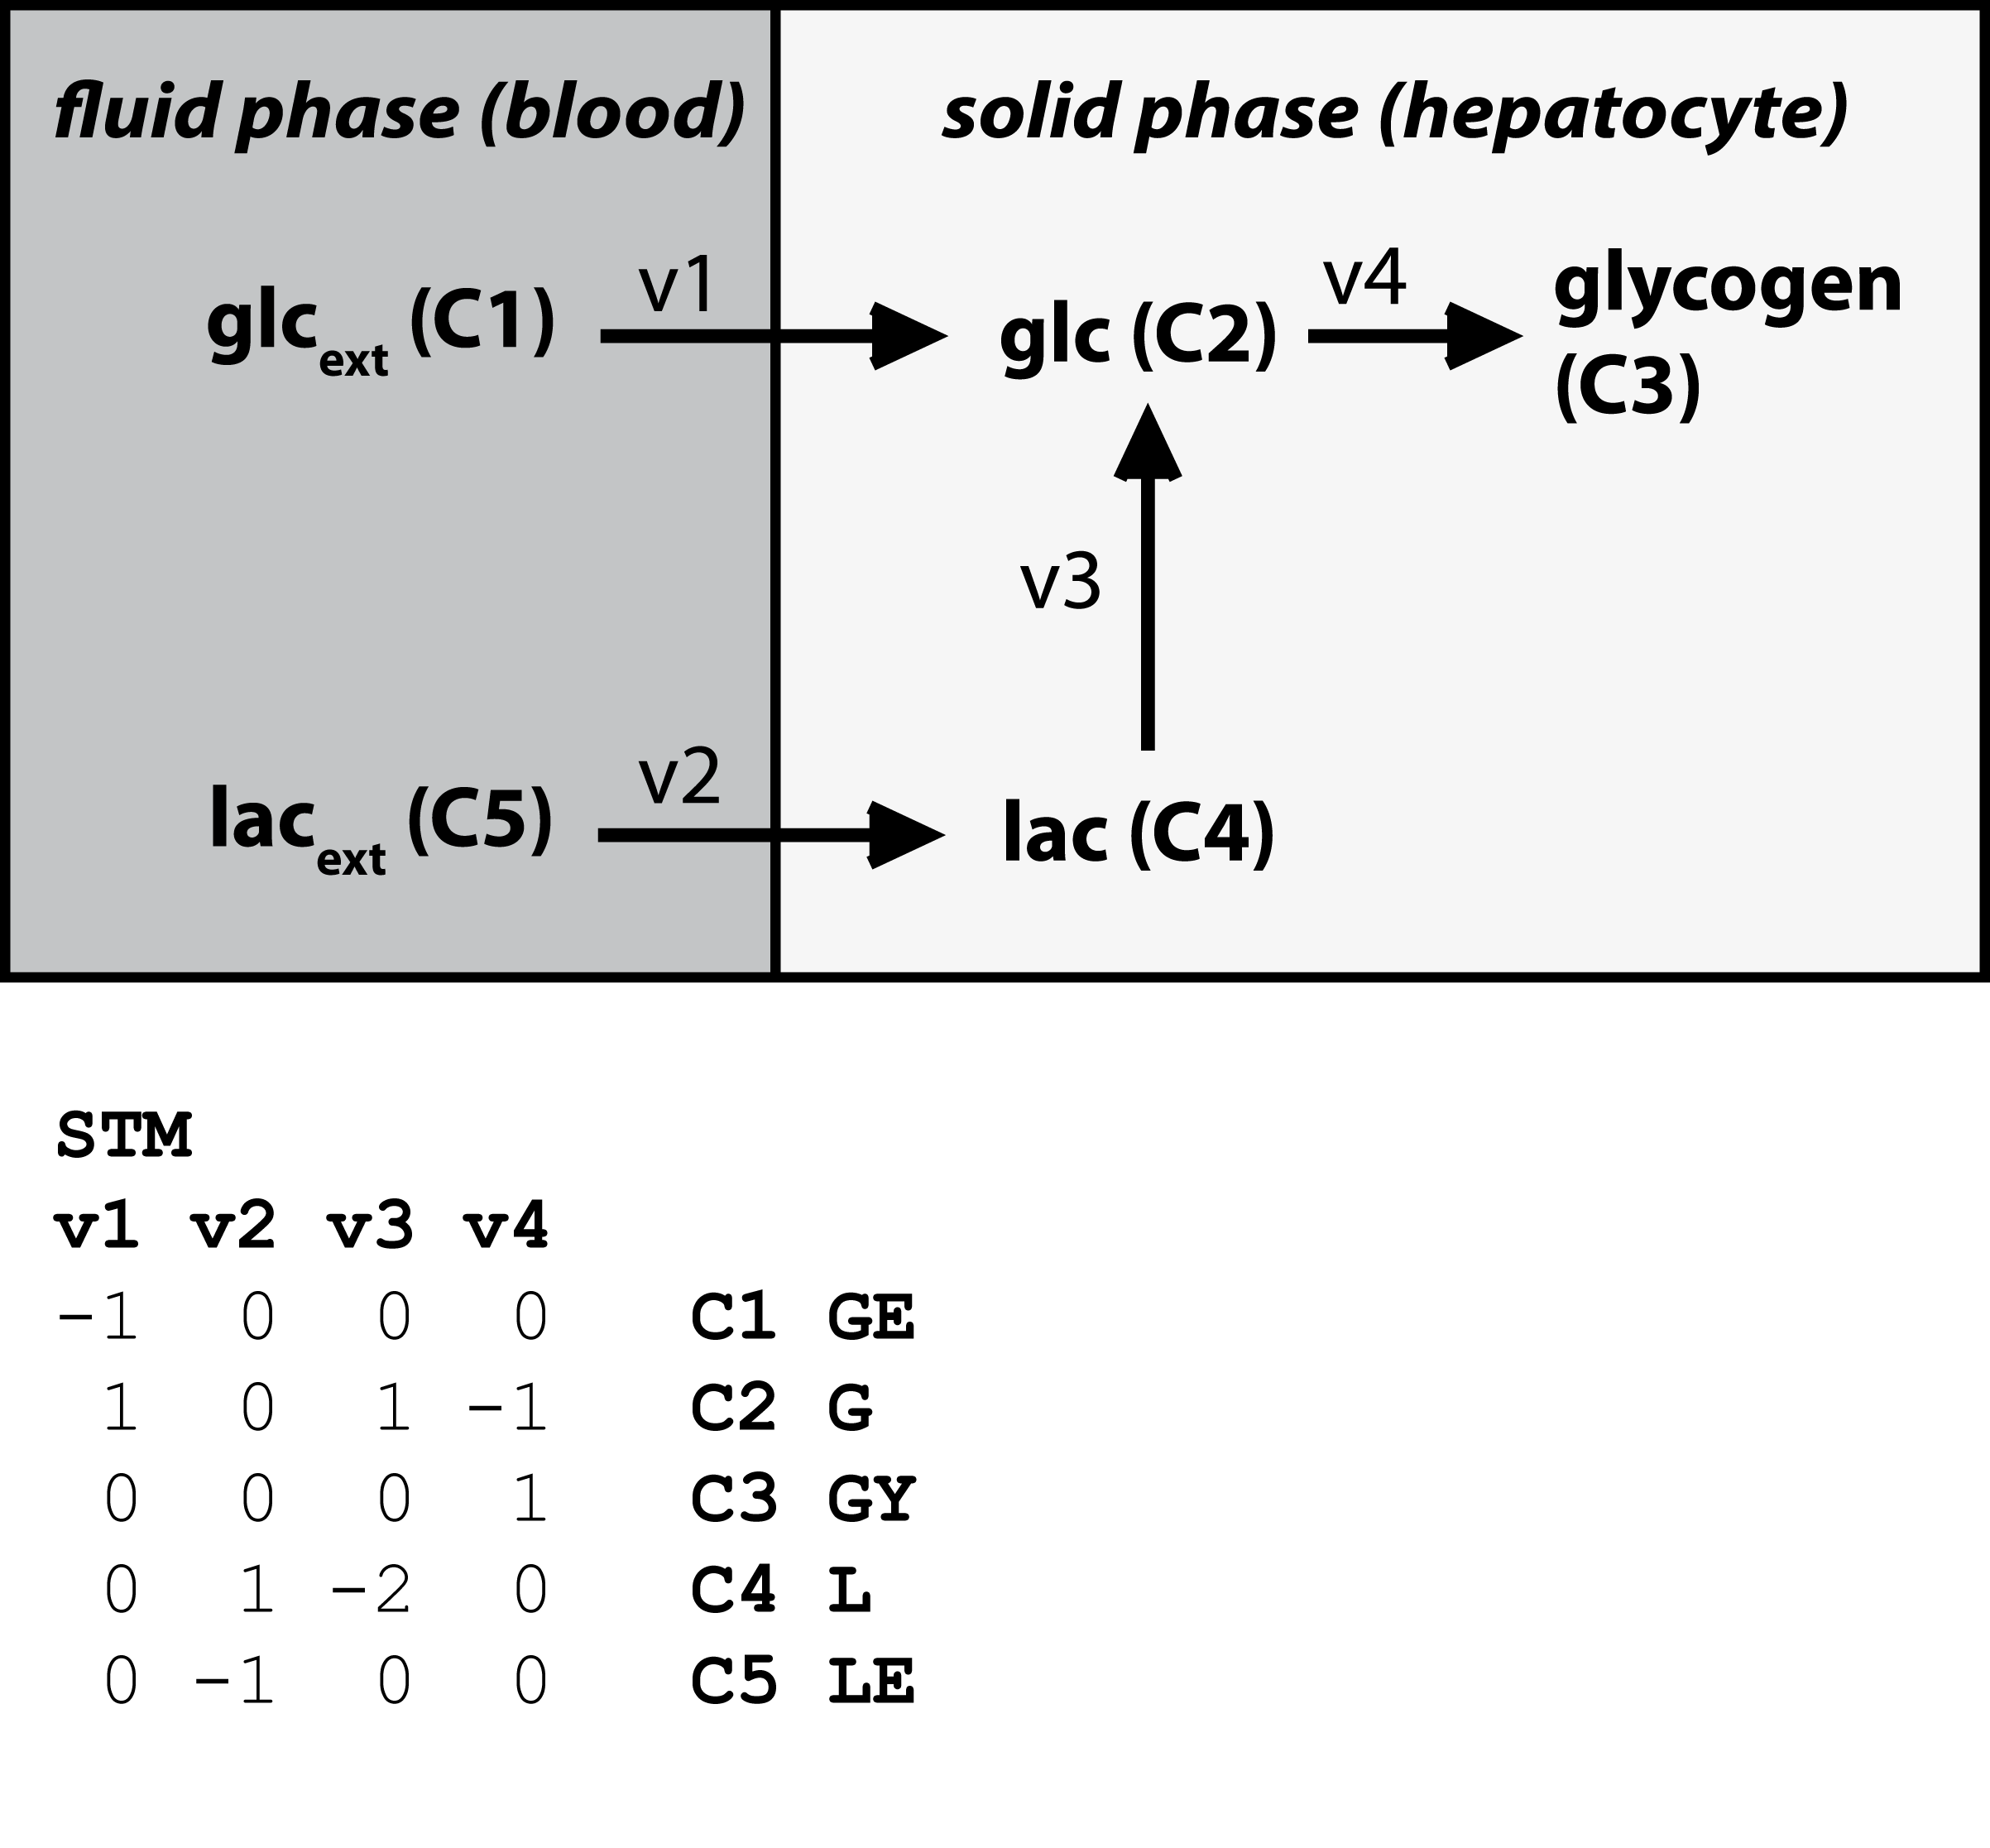
\includegraphics[width=280pt,keepaspectratio=true]{./figures/mv4_overview.png}
\caption{Kinetic model MV4 of hepatic glucose metabolism with stoichiometric matrix STM.  Model is simplified model based on detailed kinetic model of glucose metabolism with hormonal regulation and includes glycolysis, gluconeogenesis and glycogen metabolism.}
\label{fig: overview}
\end{figure}

%%%%%%%%%%%%%%%%%%%%%%%%%%%%%%%%%%%%%%%%%%%%%%%%%%%%%%%%%%%%%%%%%%%%%%%%%%%%%%%%%%%%%%%%%%%%%%%%%%%%%%%
\newpage
\begin{landscape}
\begin{multicols}{2}

\section{Rate Equations - ODE system}
\label{sec: rate_equations}
\footnotesize

\paragraph{Fitted response curves detailed model}

\begin{equation*}
x = GE;~~y = GY
\end{equation*}
\begin{equation*}
C_A = \left( \begin{array}{c}
-0.013260401508103\\
-0.000078240970095\\
   0.478235644004833\\ 
   0.000002861605817\\
   0.000932752106971\\
  -2.492569641130055\\
   0.000000166945924\\
  -0.000125285017396\\
   0.015354944655784\\
   -4.975026288067225]
\end{array} \right)
\end{equation*}
\begin{multline}
v_{gly} = \frac{90\cdot10^{-3}}{60} ( C_A(1)x^3 + C_A(2)x^2y + C_A(3)x^2 + C_A(4)xy^2 \\
		+ C_A(5)xy +C_A(6)x + C_A(7)y^3 + C_A(8)y^2 + C_A(9)y + C_A(10))
\end{multline}
\begin{equation*}
C_B = \left( \begin{array}{c}         
0.015298362033754\\
-0.000289250010776\\
-0.547536679729713\\
-0.000005684726209\\
0.010350112006466\\
6.232845830004314\\
-0.000000348461291\\
0.000282613503037\\
-0.115405862243966\\
-13.439952615163973\\
\end{array} \right)
\end{equation*}

\begin{multline}
v_{glys} =\frac{90\cdot10^{-3}}{60} ( C_B(1)x^3 + C_B(2)x^2y + C_B(3)x^2 + C_B(4)xy^2\\
	  + C_B(5)xy+C_B(6)x + C_B(7)y^3 + C_B(8)y^2 + C_B(9)y + C_B(10))    
\end{multline}

\paragraph{Adaption of gluconeogenesis rate for low lactate}
\begin{align*}
p_{LE} &= 0.1 \unit{mM} \\
n  &= 2\\
\end{align*}
\begin{equation}
v_{gly}(v_{gly}<0) = \frac{LE^n}{LE^n + p_{LE}^n} \cdot v_{gly}(v_{gly}<0);
\end{equation}

\begin{equation}
v_1 = v_{gly} + v_{glys}
\label{eq: v1}
\end{equation}


\paragraph{Adaption of glycogen metabolism rate for glycogen}
Adaption of glycogenolysis rate for low glycogen and adaption of glycogen synthesis rate for high glycogen (due to polynom fit not absolute zero).
\begin{align*}
p_{GY} &= 5 \unit{mM} \\
p_{C} &= 500 \unit{mM} \\
n  &= 2\\
\end{align*}
\begin{equation}
v_{glys}(v_{glys}<0) = \frac{GY^n}{GY^n + p_{GY}^n} \cdot v_{glys}(v_{glys}<0)
\end{equation}
\begin{equation}
v_{glys}(v_{glys}>0) = \frac{(p_{C}-GY)^n}{(p_{C}-GY)^n + p_{GY}^n} \cdot v_{glys}(v_{glys}>0) 
\end{equation}


\paragraph{$v_1$ Glucose transporter (import)}
\[ GE \leftrightarrow G \]
\begin{equation}
v_1 = v_{gly} + v_{glys}
\label{eq: v1}
\end{equation}

\paragraph{$v_2$ Lactate transporter (import)}
\[ LE \leftrightarrow L \]
\begin{equation}
v_2 = - 2 \cdot v_{gly}
\label{eq: v2}
\end{equation}

\paragraph{$v_3$ Gluconeogenesis/glycolysis}
\[ 2 L \leftrightarrow G \]
\begin{equation}
v_3 = -v_gly
\label{eq: v3}
\end{equation}

\paragraph{$v_4$ Glycogen synthesis/glycogenolysis}
\[ C \leftrightarrow CE \]
\begin{equation}
v_4 = v_{glys}
\label{eq: v4}
\end{equation}

\end{multicols}
\end{landscape}

%%%%%%%%%%%%%%%%%%%%%%%%%%%%%%%%%%%%%%%%%%%%%%%%%%%%%%%%%%%%%%%%%%%%%%%%%%%%%%%%%%%%%%%%%%%%%%%%
\section{Source and sink terms}
Change of concentration in timestep DT:
\begin{equation}
 c_i(t+DT) = c_i(t) + DT \cdot F_i \cdot V
\end{equation}
F is change in concentration in calculated for unit volume (1 $L$) in the timestep DT. The actual change in concentration results from multiplication with Volume V and size of timestep DT. F > 0 : concentration increases, F < 0 : concentration decreases.
\begin{equation}
 [F] = \frac{\unit{mmol}}{\unit{L}} \cdot \frac{1}{\unit{Ls}} = 10^{-3} \frac{\unit{mol}}{\unit{m³}} \cdot \frac{1}{\unit{m³s}}
\end{equation}


%%%%%%%%%%%%%%%%%%%%%%%%%%%%%%%%%%%%%%%%%%%%%%%%%%%%%%%%%%%%%%%%%%%%%%%%%%%%%%%%%%%%%%%%%%%%%%%%
\section{Simulations}
\label{sec: simulations}
 
\begin{figure}[htp]
 \centering
 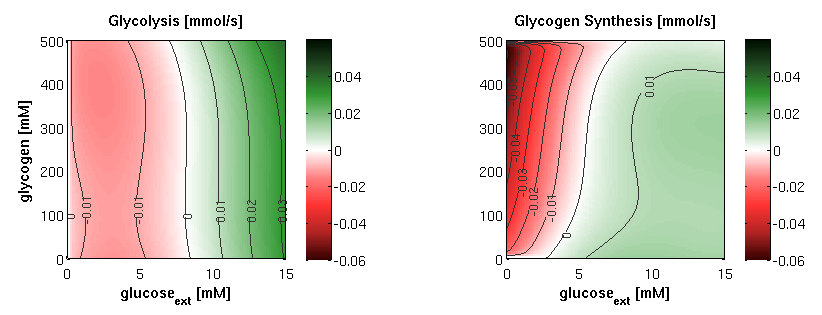
\includegraphics[width=400pt,keepaspectratio=true]{./figures/mv4_response_curves.png}
\caption{MV4 response depending on external glucose and the internal glycogen state. Gluconeogenesis and glycogen synthesis. Response curves result from multidimensional polynom fit of order 4 or higher to the full model.}
\label{fig: response}
\end{figure}

\begin{figure}[htp]
 \centering
 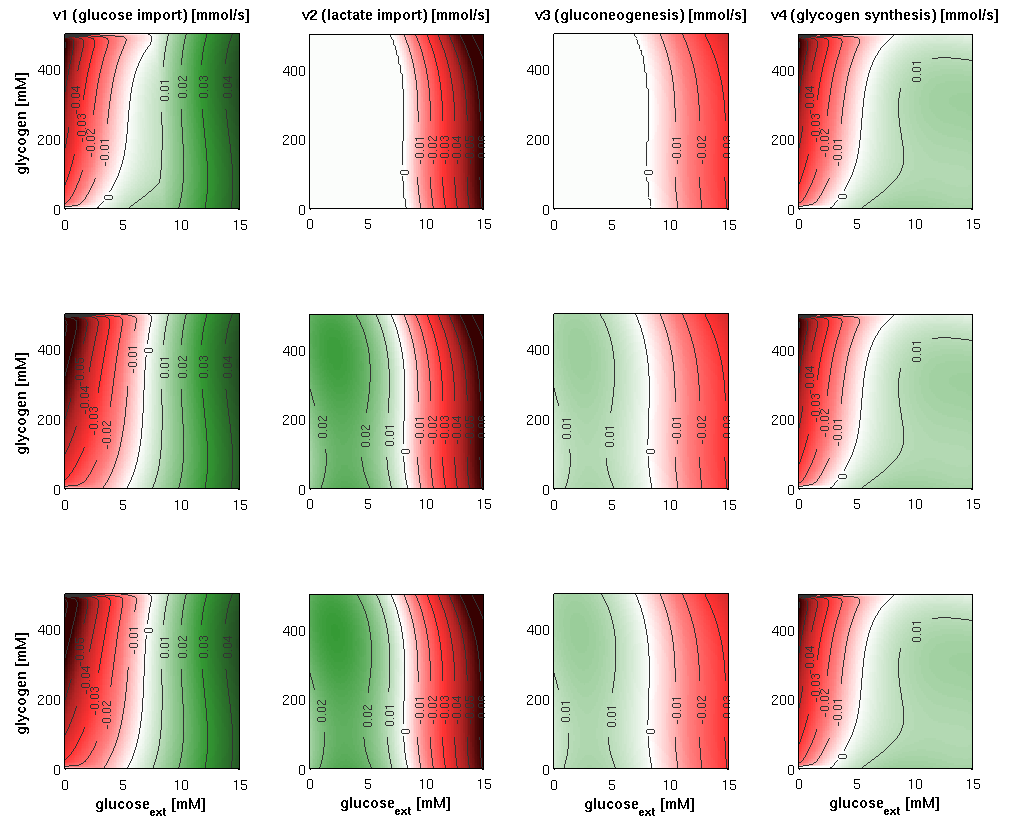
\includegraphics[width=400pt,keepaspectratio=true]{./figures/mv4_model_behavior.png}
\caption{MV4 full model response depending on external glucose, external lactate and glycogen content.}
\label{fig: behavior}
\end{figure}

\begin{figure}[htp]
 \centering
 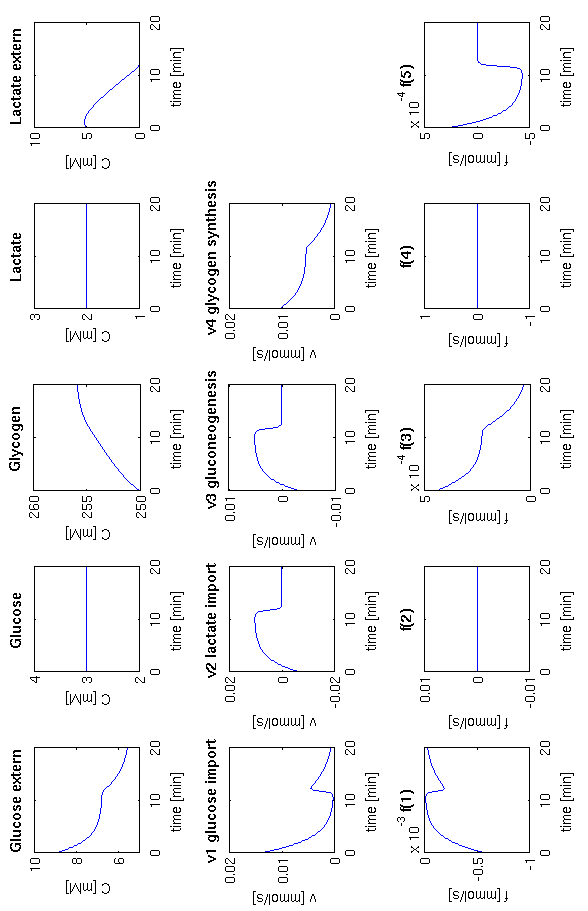
\includegraphics[width=350pt,keepaspectratio=true]{./figures/mv4_sim1.png}
\caption{Simulation: $c_{init} = [9~3~250~2~5]mM$, $ t= 0:1:1200s$. External glucose, external lactate and glycogen are variable}
\label{fig: sim1}
\end{figure}
